\documentclass[12pt,a4paper]{article}
\usepackage{hw}

\graphicspath{ {.} }
\setlength\parindent{0pt}

\begin{document}
\qtitle{10.1}
Assume there is 1L Tc-99m solution, \\
$N_0=10*10^{-12}mole/L*1L*6.022*10^{23}atoms/mole=6.022*10^{12}atoms$ \\
According to equation 10.6, \\
$t_{1/2}=ln2/\lambda\rightarrow\lambda=ln2/t_{1/2}=ln2/(6*3600s)=3.21*10^{-5}s^{-1}$ \\
Then $A=-dN/dt=-d(N_0exp(-\lambda t))/dt=N_0\lambda exp(-\lambda t)\\
=6.022*10^{12}atoms*3.21*10^{-5}s^{-1}*exp(-3.21*10^{-5}t)\\
=1.93*10^8exp(-3.21*10^{-5}t) [Bq]$

If there is $k$L solution, the previous value should by multiplied by $k$ fold.

\newpage
\qtitle{10.2}
\textbf{a).} For 1st compartment, $\Delta m_1(t)=-\Delta t q c_1(t) step(t)$. \\
As example 10.1.3, we have $c_1(t)=c_0exp(-qt/V_1)step(t)$

\vspace{0.5cm}
\textbf{b).} For 2st compartment, $\Delta m_2(t)=\Delta t q c_1(t)step(t)-\Delta tq c_2(t)step(t)$ \\
For $t>0$ and $m_2(t)=c_2(t)*V_2$, \\
$\cfrac{dc_2}{dt}=(qc_1(t)-qc_2(t))/V_2\rightarrow\dot{c_2(t)}+\cfrac{q}{V_2}c_2(t)=\cfrac{q}{V_2}c_1(t)$ \\
So $c_2$ is a first-order nonautonomous system, then according to equation 10.16, \\
$h(t)=exp(-qt/V_2)step(t)$ and $f(t)=q/V_2*c_1(t)$, then\\
$c_2(t)=\infint dt' h(t')f(t-t')\\
=q/V_2\bint{0}{\infty} dt'exp(-qt'/V_2)*c_0exp(-q(t-t')/V_1)step(t-t')\\
=\cfrac{qc_0}{V_2}exp(-qt/V_1)\bint{0}{t}dt' exp(q/V_1-q/V_2)t'\\
=\cfrac{qc_0}{V_2}exp(-qt/V_1)\cfrac{1}{q/V_1-q/V_2}(exp((q/V_1-q/V_2)t)-1)\\
=\cfrac{c_0V_1}{V_2-V_1}(exp(-qt/V_2)-exp(-qt/V_1))\\
=\cfrac{c_0}{1/a-1}(exp(-aqt/V_1)-exp(-qt/V_1))$\\
Therefore, the engineering paramters of this system is $\cfrac{V_1}{V_2-V_1}$, $q/V_1$ and $q/V_2$

\begin{figure}[!ht]
    \centering
    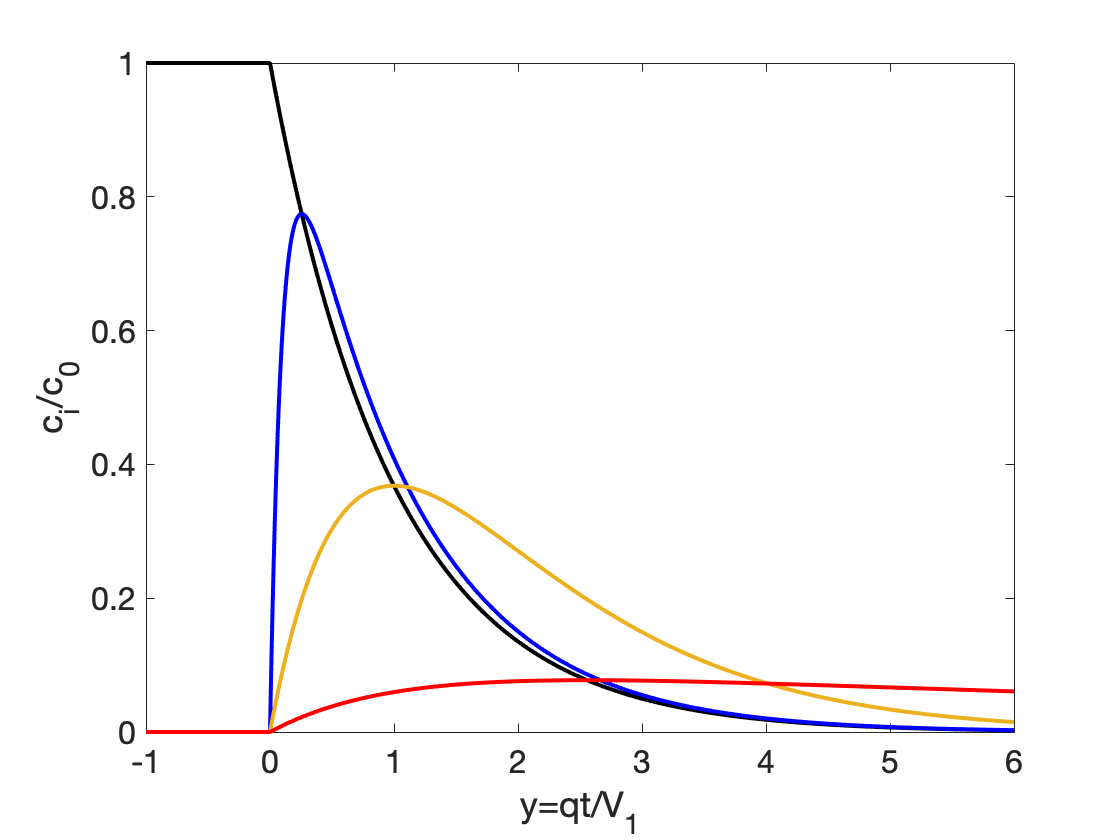
\includegraphics[width=\textwidth]{hw10_2.png}
    \caption{$c_1$ and $c_2$ of two compartment system. black curve: $c_1$; \textcolor{blue}{blue curve}: $c_2;a=10$; \textcolor{orange}{orange curve}: $c_2;a=1+\epsilon$; \textcolor{red}{red curve}: $c_2;a=0.1$}
\end{figure}

\clearpage
\qtitle{10.4}
\textbf{(a)} According to example 10.3.2, for Mo-99:\\
$A_M(t)=-\dot{N}_M(t)=\lambda_MN_{0M}exp(-\lambda_Mt)$

For Tc-99m, $N_T(t)=\cfrac{\lambda_MN_{0M}}{\lambda_T-\lambda_M}(exp(-\lambda_Mt)-exp(-\lambda_Tt))$ \\
$A_T(t)=-\lambda_TN_T(t)=-\cfrac{\lambda_T\lambda_MN_{0M}}{\lambda_T-\lambda_M}(exp(-\lambda_Mt)-exp(-\lambda_Tt))$

In order to maximize Tc-99m activity recovery, we need to dilute the Tc-99m from the column when its number reaches the peak, which is to extract Tc-99m once the system reaches the equilibrium status. 

For the first dilution when $N_{0T}=0$, the first time that the system has equilibrium status is when $\dot{A}_T(t_1)=0$:\\ 
$-\lambda_Mexp(-\lambda_Mt_1)+\lambda_Texp(-\lambda_Tt_1)=0\rightarrow t_1=\cfrac{ln(\lambda_M/\lambda_T)}{\lambda_M-\lambda_T}$

For the rest dilutions, since the extraction efficiency is 0.9, there is remaining Tc-99m and decreased Mo-99 for the next stage. \\
$N'_{0T}=0.1*N(t_{milk});N'_{0M}=N_{0M}exp(-\lambda_Mt_{milk})\\
 N(t)=\lambda_MN_M(t)-\lambda_T N_T(t)+N'_{0T}$

Then $f(t)=\lambda_MN_M(t)+N'_{0T}\rightarrow\\
N'_T(t)=\infint dt'h(t')f(t-t')
=\lambda_MN'_{0M}\infint dt' exp(-\lambda_Tt')step(t')exp(-\lambda_M(t-t'))step(t-t')+\infint dt' exp(-\lambda_Tt')step(t')N'_{0T}\\
=\cfrac{\lambda_MN'_{0M}}{\lambda_T-\lambda_M}(exp(-\lambda_Mt)-exp(-\lambda_Tt))+N'_{0T}/\lambda_T$

Then $A'_T(t)=-\lambda_TN'_T(t)=-\cfrac{\lambda_T\lambda_MN'_{0M}}{\lambda_T-\lambda_M}(exp(-\lambda_Mt)-exp(-\lambda_Tt))-N'_{0T}$. 

It's easy to know the time to reach equilibrium status doesn't change. That is $t_{milk}=\cfrac{ln(\lambda_M/\lambda_T)}{\lambda_M-\lambda_T}$

For Mo-99, $\lambda_M=ln(2)/t_{1/2M}=0.0105$; For Tc-99m, $\lambda_T=ln(2)/t_{1/2T}=0.1155$. So $\Delta t_{milk}=22.83h$

Use the following code, we could get the activity dynamic figure along time. 
\begin{lstlisting}
t0=-5:0.1:0;t1=0.1:0.1:150;t=-5:0.1:150;
lamM=log(2)/66;lamT=log(2)/6;
c1_0=ones(1, length(t0))*lamM;
c2_0=zeros(1, length(t0));
N0M=1;N0T=0;
c1 = lamM*exp(-lamM*t1)*N0M;
c1_z = cat(2, c1_0, c1);
figure;
plot(t, c1_z, 'k-', 'linewidth', 2); hold on;
Tmilk=round(log(lam_m/lam_T)/(lam_m-lam_T), 1);
n_milk=0;
for ti=t1
    c2 = lamT*lamM*N0M/(lamT-lamM)*(exp(-lamM*(ti-Tmilk*n_milk))-exp(-lamT*(ti-Tmilk*n_milk)))+N0T;
    c2_0(end+1)=c2;
    if mod(ti, Tmilk) == 0
        n_milk=n_milk+1;
        N0M=exp(-lamM*ti)*N0M;
        N0T=0.1*c2;   
    end
end
\end{lstlisting}
\begin{figure}[!ht]
    \centering
    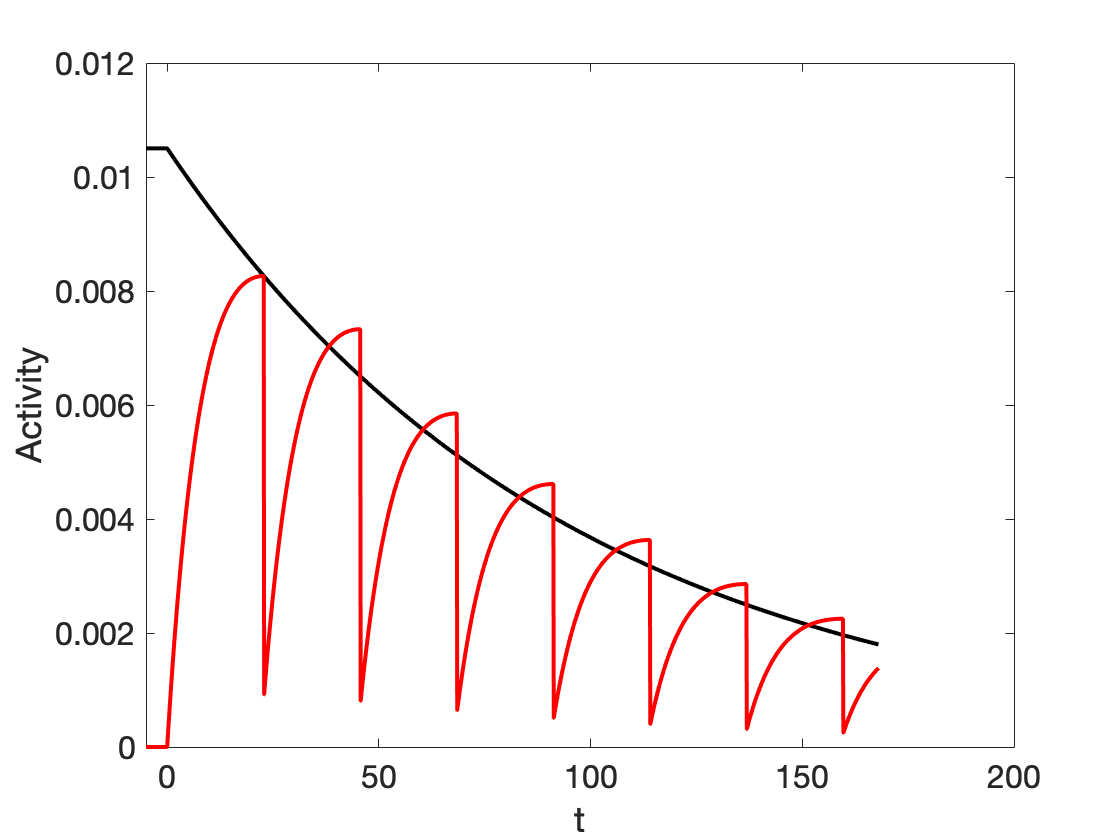
\includegraphics[width=0.8\textwidth]{hw10_4.png}
    \caption{Activity of Mo-99 and Tc-99m along time. black: M0-99; red: Tc-99m}
\end{figure}

\textbf{(b)} The total activity produced in a week is $A_{Ttotal}=\bint{0}{24\times 7}A_T(t)dt=0.6233N_{0M}$, $A_{Tmilk}=0.9*\sum_{i=1}^7A'_{Ti}(22.8)=0.0313N_{0M}$. Recoveray fraction is $r=0.0313/0.6233=5.02\%$

\newpage 
\qtitle{10.5}
To find the best parameters to fit the data, we use MSE error to estimate the real data with predicted data. Since both lynx or rabbit data could be used as independent variable to predict another one, we define the MSE as $MSE=(MSE_{x_1=lynx}+MSE_{x_1=rabbit})/2$. Then we use grid search to find the best $\alpha, \beta, \gamma, k$. Here is the code. We limit the search range for $\alpha$ is [0.01, 0.03]; $\beta$ is [0.1, 0.7]; $\gamma$ is [0.8, 1]; $k$ is [0.1, 0.7].  

\begin{lstlisting}
lynx=[4.0 6.1 9.8 35.2 59.4 41.7 19.0 13.0 8.3 9.1 7.4 8.0 12.3 19.5 45.7 51.1 29.7 15.8 9.7 10.1 8.6];
rab=[30.0 47.2 70.2 77.4 36.3 20.6 18.1 21.4 22.0 25.4 27.1 40.3 57.0 76.6 52.3 19.5 11.2 7.6 14.6 16.2 24.7];
min_disc = 1e10;
for k=0.1:0.02:0.7
    for alpha=0.01:0.002:0.03
        for gamma=0.8:0.02:1
            for beta=0.1:0.02:0.7
                theta=[k alpha;gamma beta];
                Ns=[k/alpha;beta/(alpha*gamma)];
                N0=[4;30];
                trange=[0 20];
                [tt,N]=ode45(@(tt,N) lotka1(tt, N, theta), trange, N0);
                xi=[N(:,1)-Ns(1),N(:,2)-Ns(2)];
                x1max=max(N(:, 1)-Ns(1));x2max=max(N(:,2)-Ns(2));
                a=x2max^2/Ns(2);
                b=x1max^2/gamma/Ns(1);
                x1_l=lynx-Ns(1);
                x2_l=real(sqrt((a-x1_l.^2/gamma/Ns(1))*Ns(2)));
                x2_r = rab - Ns(2);
                x1_r = real(sqrt((b-x2_r.^2/Ns(2))*gamma*Ns(1)));
                rab_disc = abs(rab-Ns(2));
                pred_rab_disc = x2_l-rab_disc;
                % mse for predict rabit
                rab_d = sqrt(sum((pred_rab_disc - rab_disc).^2)/length(rab));
                lynx_disc = abs(lynx - Ns(1));
                pred_lynx_disc = x1_r - lynx_disc;
                % mse for predict lynx
                lynx_d = sqrt(sum((pred_lynx_disc-lynx_disc).^2)/length(lynx));
                disc = lynx_d + rab_d;
                if disc < min_disc
                    min_disc = disc;
                    min_alpha=alpha;min_beta=beta;min_gamma=gamma;min_k=k;
                    min_tt=tt;min_xi=xi;min_N=N;min_Ns=Ns;
                end
            end
        end
    end
end
\end{lstlisting}

In this setting, we obtain the min MSE value as 38.47 ($MSE_{x_1=lynx}=19.28;MSE_{x1=rabbit}=19.18$) when $\alpha=0.014, \beta=0.54,\gamma=1,k=0.28$. 
\begin{figure}[!ht]
    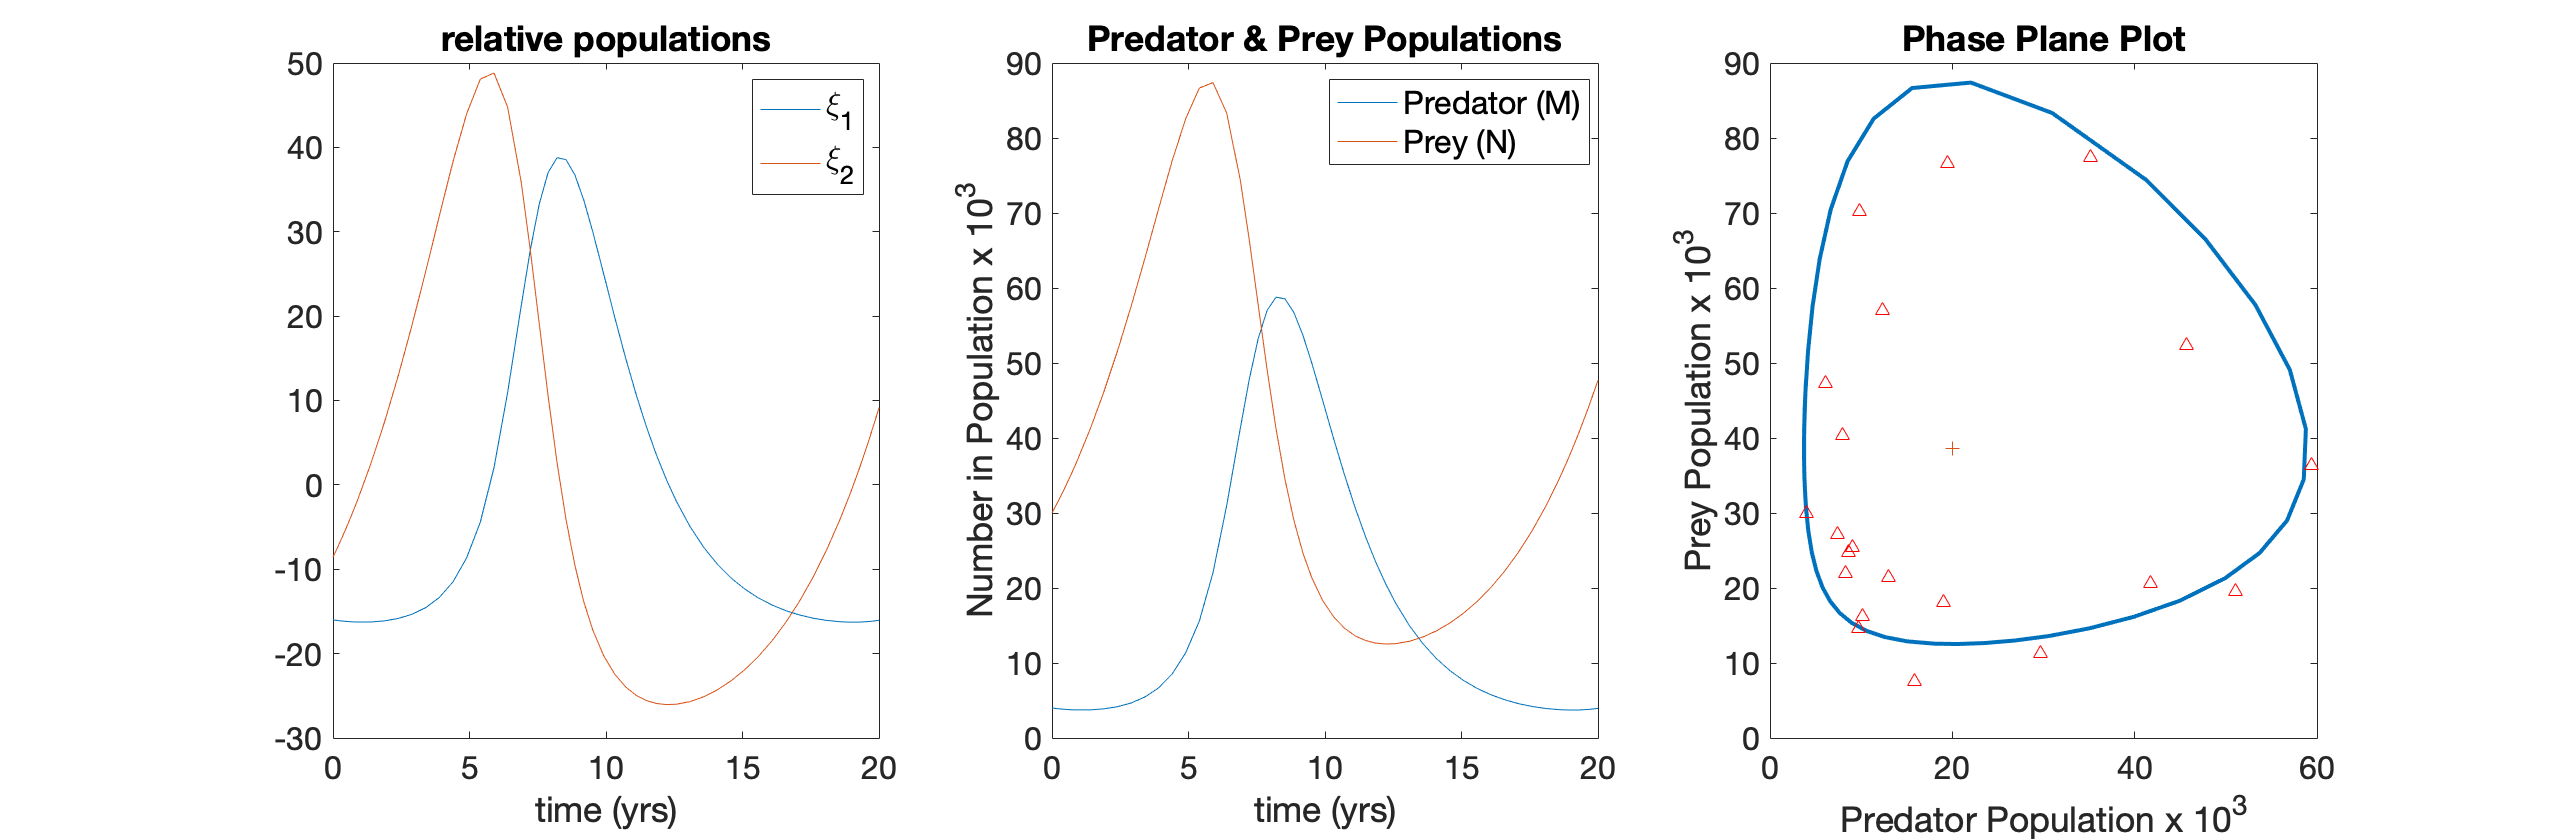
\includegraphics[width=\textwidth]{hw10_5_b.png}
    \caption{Rabbit-Lynx dynamic variation along time and its trajectories through state space.($\alpha$=0.014)}
\end{figure}

However, if we stick $\alpha=0.02$ and $\gamma=1$ and search for optimal $\beta$ and $k$. We would get the sub-optimal MSE value as 39.66 ($MSE_{x_1=lynx}=18.75;MSE_{x1=rabbit}=20.91$) when $\alpha=0.02, \beta=0.7,\gamma=1,k=0.4$, while the trajectory curve seems to fit the data better (\textcolor{red}{red} triangle). 
\begin{figure}[!ht]
    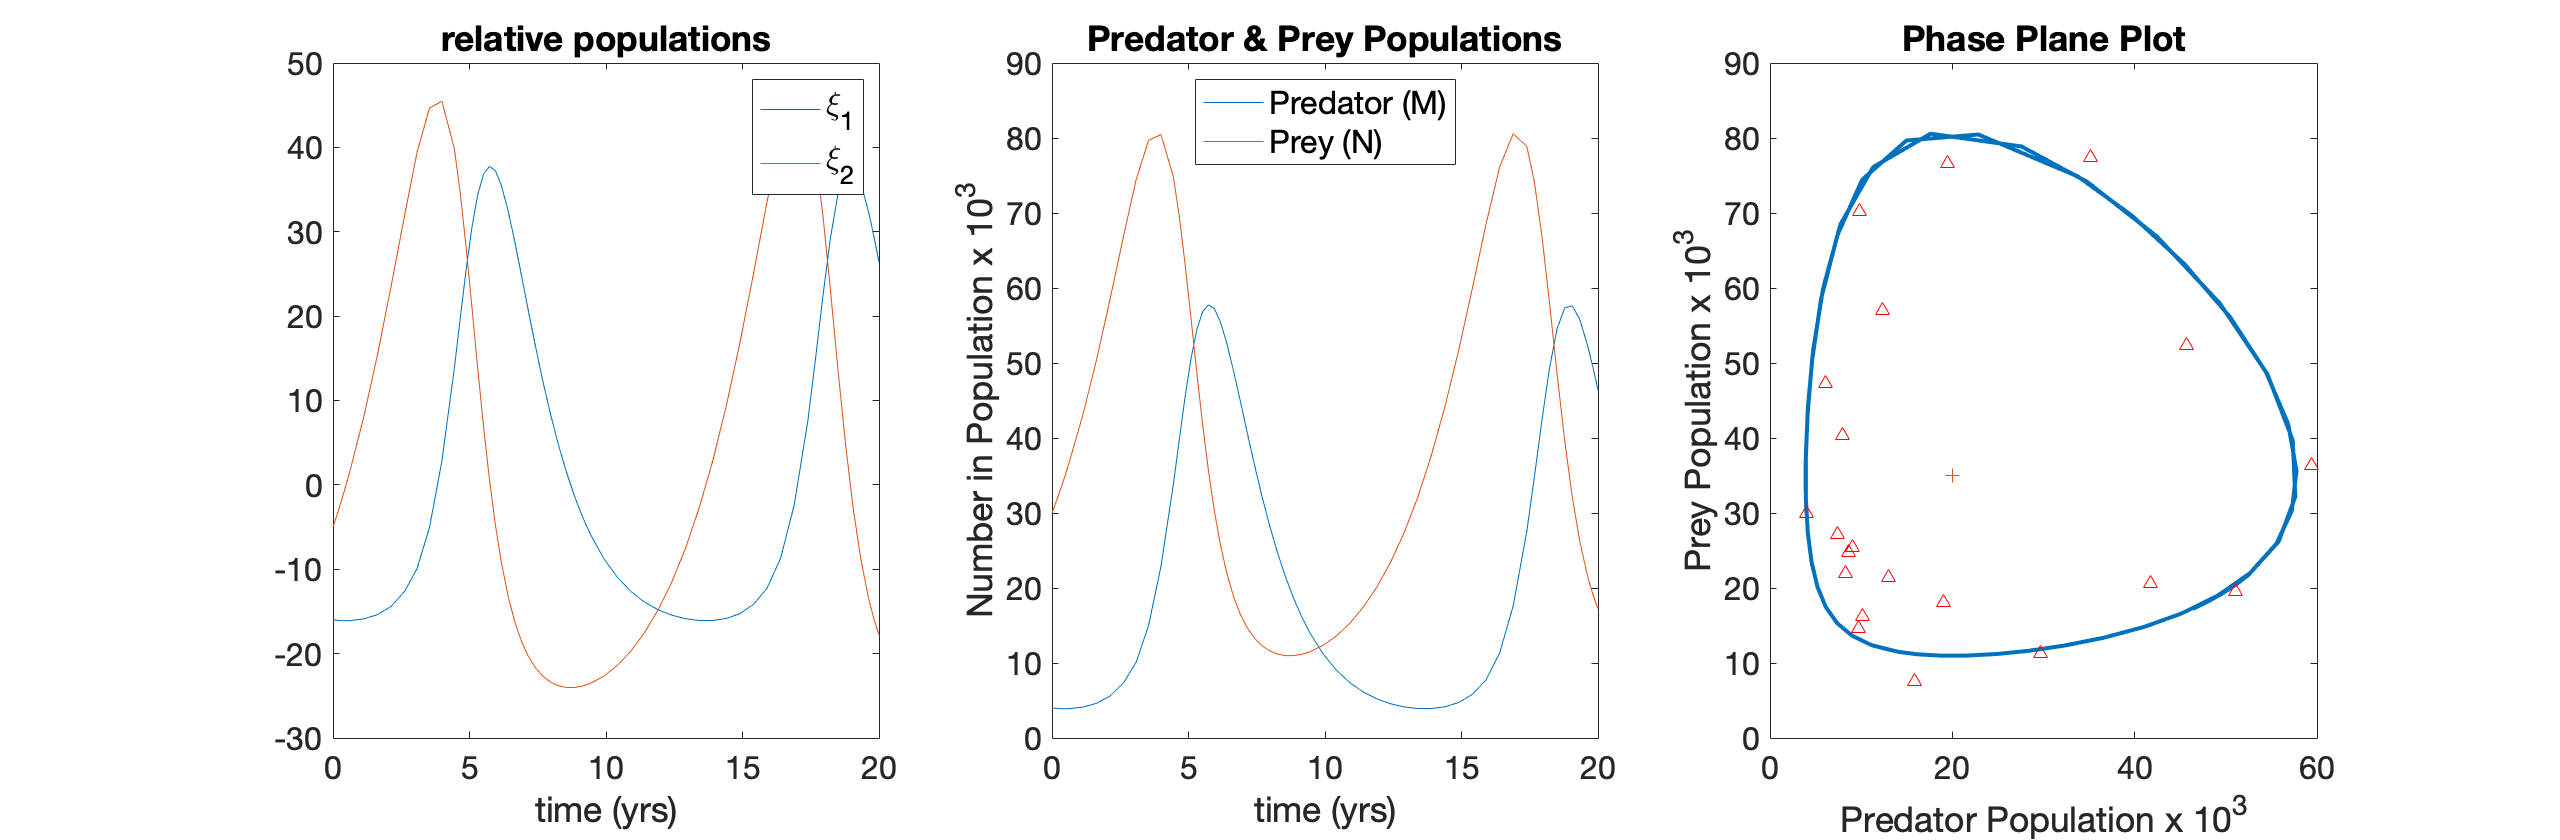
\includegraphics[width=\textwidth]{hw10_5_a.png}
    \caption{Rabbit-Lynx dynamic variation along time and its trajectories through state space.($\alpha$=0.02)}
\end{figure}

Anyway, both parameters could fit the data well but the later one has higher prey reproduce rate (k) and predator die rate ($\beta$). It's intuitive to see that the population oscillation would has short period and higher frequency, because the population could increase or decrease faster. This meets the trend shown in the figures. 

\newpage
\qtitle{10.6}
In the prey-predator model, the 2D Lotka-Volterra equations are as equation 10.34: \\
$\dot{\xi_1}(t)=\gamma\alpha N(t)M(t)-\beta M(t)-M_s\\
\dot{\xi_2}(t)=kN(t)-\alpha N(t)M(t)-N_s$\\
And the Jacobian matrix is $\mathbf{A}=\newvec{\gamma\alpha N_s-\beta&\gamma\alpha M_s\\-\alpha N_s & k-\alpha M_s}$

Given $\mathbf{N_s}=\newvec{M_s\\N_s}=\newvec{k/\alpha\\\beta/\alpha\gamma}$ and $\alpha=0.02;\beta=0.6;\gamma=1;k=0.5$, to compute eigenvalues of $\mathbf{A}$, \\$det(\mathbf{A-\lambda\mathbf{I}})=\newdet{\gamma\alpha N_s-\beta-\lambda&\gamma\alpha M_s\\-\alpha N_s & k-\alpha M_s-\lambda}=\newdet{-\lambda&0.5\\-0.6&-\lambda}=0$

We get $\lambda_1=\sqrt{0.3}i;\lambda_2=-\sqrt{0.3}i$, which are conjugate complex numbers without real parts. \\
$\mathbf{\Lambda}=\newvec{\sqrt{0.3}i&0\\0&\sqrt{0.3}i}$ and eigenvectors are $\mathbf{u_1}=\newvec{\sqrt{0.3}\\-0.6i}u;\mathbf{u_2}=\newvec{\sqrt{0.3}\\0.6i}v$\\
$\mathbf{U}=\newvec{\sqrt{0.3}&\sqrt{0.3}\\-0.6i&0.6i}$
As equation 10.13 does, we have: \\
$\xi_1(t)=\sqrt{0.3}u(exp(\sqrt{0.3}it)+exp(-\sqrt{0.3}it))\\
\xi_2(t)=0.6vi(exp(\sqrt{0.3}it)-exp(-\sqrt{0.3}it))$

Apply Eular's equation and let $\Omega_0=|\lambda|=\sqrt{k\beta}$, \\
$\xi_1(t)=2\sqrt{0.3}ucos(\Omega_0t)\\
\xi_2(t)=2*0.6visin(\Omega_0t)$

In this example, $\xi_{1max}=2.7;\xi_{2max}=3$. So let $u=v=2.5$, we have: \\
$\xi_1(t)=2.7cos(\Omega_0t)=\xi_{1max}cos(\Omega_0t)=\xi_{1max}\mathfrak{R}\{exp(\lambda_1t)\}\\
\xi_2(t)=3sin(\Omega_0t)=\xi_{2max}sin(\Omega_0t)=\xi_{2max}cos(\Omega_0t+\pi/2)=\xi_{2max}\mathfrak{I}\{exp(\lambda_2t)\}$, which is equation 10.42.

\newpage
\qtitle{10.7}
After time $t_0$, the death rate of predator $\beta'=\beta-\kappa$, where $\beta>0,\kappa<0$. So the death rate of predator increases after $t_0$, consistent with the operation that 25 animals was taken away each year. 

The equilibrium status is $\mathbf{N_s}\newvec{M_s\\N_s}=\newvec{k/\alpha\\(\beta-\kappa)/\alpha\gamma}>\newvec{k\alpha\\\beta/\alpha\gamma}$, so the equilibrium point in trajectories space move up. 

Then use the $\beta'$ and population $\newvec{M(t=30)\\N(t=30)}$ to compute the LV equations again: 
\begin{lstlisting}
k=0.5;alpha=0.02;
gamma=1;beta=0.6;
kappa=-0.025;
theta1=[k alpha;gamma beta];
theta2=[k alpha;gamma beta-kappa]; % params after t=30
Ns1=[k/alpha;beta/(alpha*gamma)];
Ns2=[k/alpha;(beta-kappa)/alpha/gamma]; % equilibrium point after t=30
N00=[23;32];
trange=[0 30];  % initial population at t=0
[tt1,N1]=ode45(@(tt,N) lotka1(tt, N, theta1), trange, N00);
N01=[N1(end,1);N1(end,2)]; % initial population at t=30
[tt2, N2]=ode45(@(tt,N) lotka1(tt, N, theta2), trange, N01);
\end{lstlisting}
\begin{figure}[!ht]
    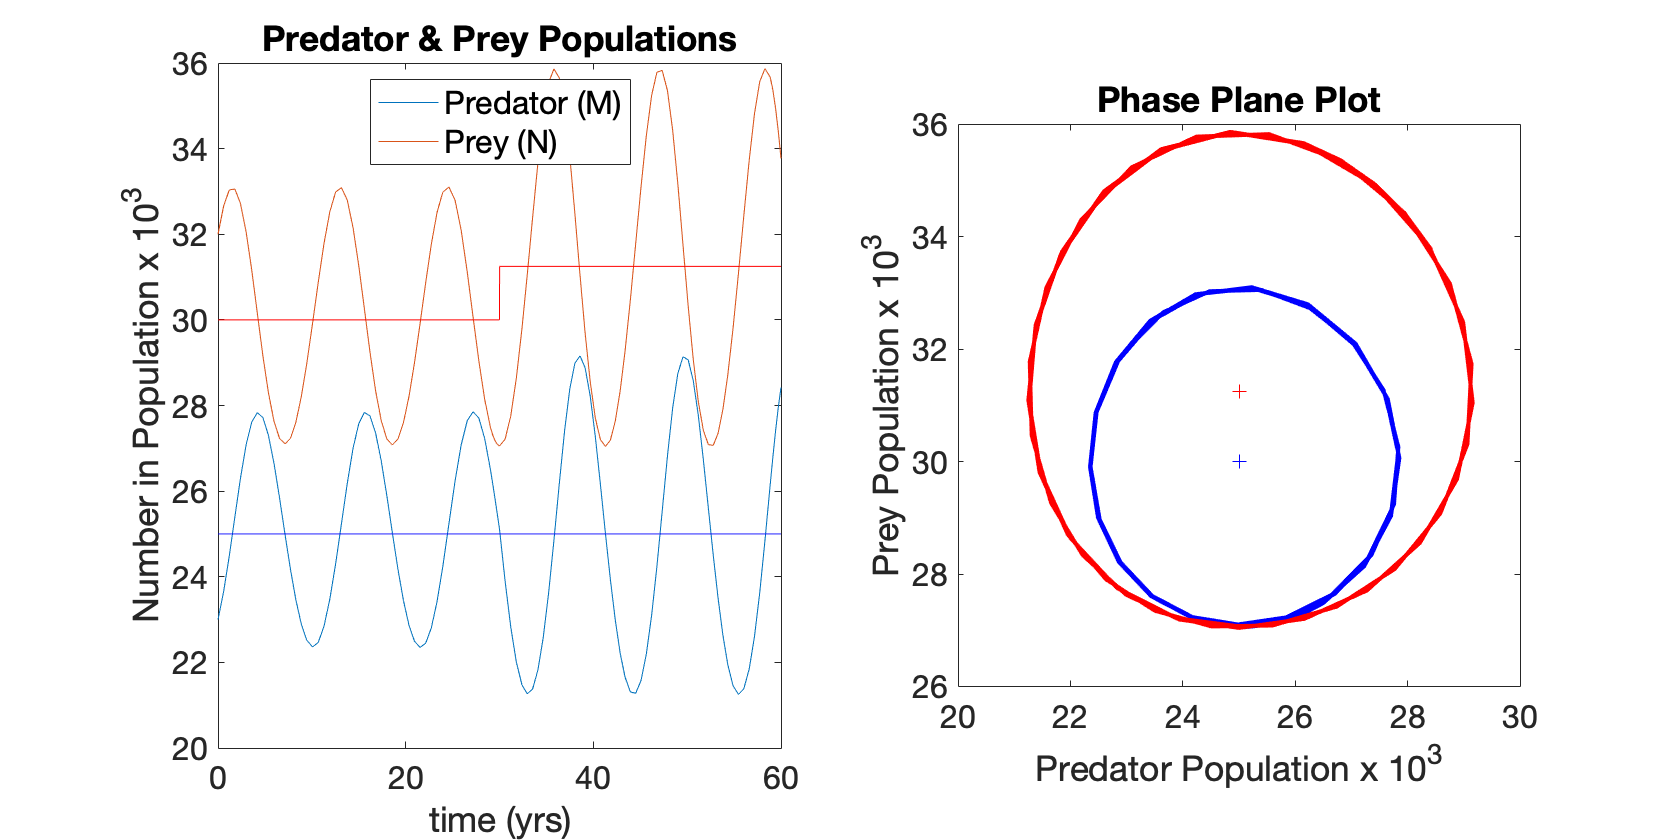
\includegraphics[width=\textwidth]{hw10_7.png}
    \caption{Solutions of LV system when $\kappa=-0.025$.\textcolor{blue}{blue}: initial trajectory; \textcolor{red}{red}: trajectory after applying $\kappa$}
\end{figure}

According to 10.42, the magnitude of eigenvalues is the radial frequency of oscillation, $|\lambda|=\sqrt{k\beta}$. So the frequency of the predator-prey population oscillation increases as shown in the figure. Since the max population and $\xi_{max}$ increases, the trajectory space is larger. Except for the minimum population of prey changes little, minimum population of predator and maximum population of prey and predator all increase. It's intuitive that less predator corresponds to the higher prey within in a short period. 

However, this is different with what the textbook shows. To match that where $N_s$ decrease after applyting $\kappa$ to $\beta$, $\kappa$ should be positive. Then we set $\kappa=0.025$ and execute the script again. We have:

\begin{figure}[!ht]
    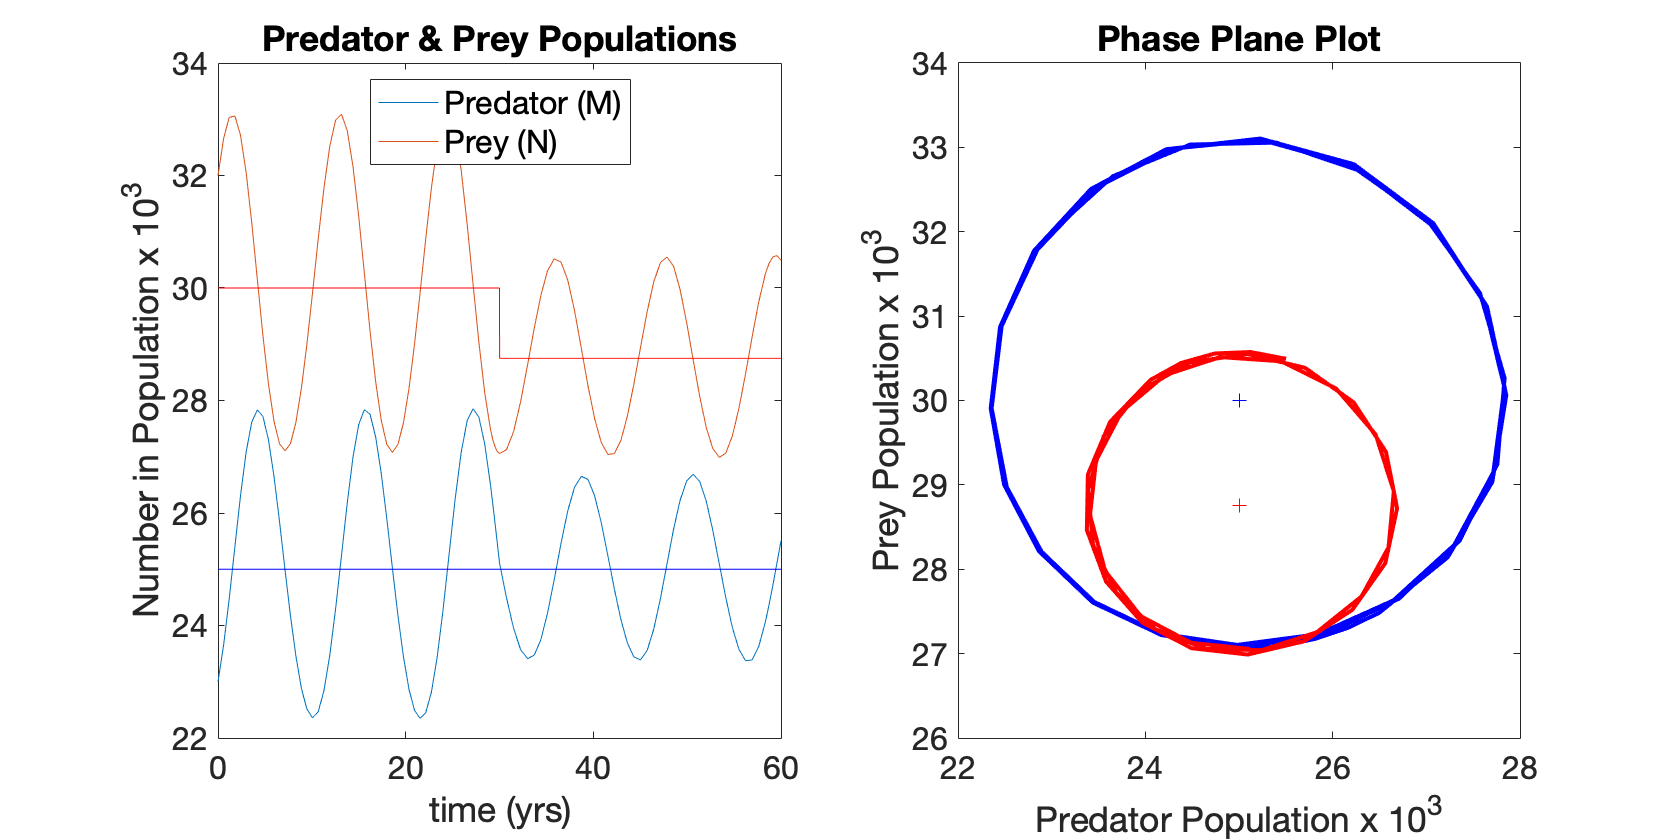
\includegraphics[width=\textwidth]{hw10_7_b.png}
    \caption{Solutions of LV system when $\kappa=0.025$.\textcolor{blue}{blue}: initial trajectory; \textcolor{red}{red}: trajectory after applying $\kappa$}
\end{figure}

In this case, we have the same trend as in the textbook. That is to reduce the death of predator to decrease the oscillation frequency and magnitude. 

\newpage
\qtitle{10.8}
\textbf{(a)} 
SIRS model equations: \\
\begin{align*}
    \dot{S} &= -\alpha SI+kR\\
    \dot{I} &= \alpha SI - \gamma I\\
    \dot{R} &= \gamma I - kR
\end{align*}
where $\alpha$ is the infection rate of transmiting disease between susceptible people and infectious people; $\gamma$ is recovery rate; $k$ is the return-to-susceptible rate when people lose immunity. 

\textbf{(b)}
According to equations in (a), we set SIRS model function and parameters $\theta$ as: 

\begin{lstlisting}
theta=[alpha;gamma;k];
...
function z=SIRS(t,y,p)
    z=([-p(1)*y(2),0,p(3);p(1)*y(2),-p(2),0;0,p(2),-p(3)])*y;
end
\end{lstlisting}

Since $k\in[0,1]$, we choose 8 k values to see their effect. $k_i=[0 0.01 0.05 0.1 0.25 0.5 0.75 1]$. When $k=0$, the SIRS model should have same outcome as SIR model. 

\begin{figure}[!ht]
    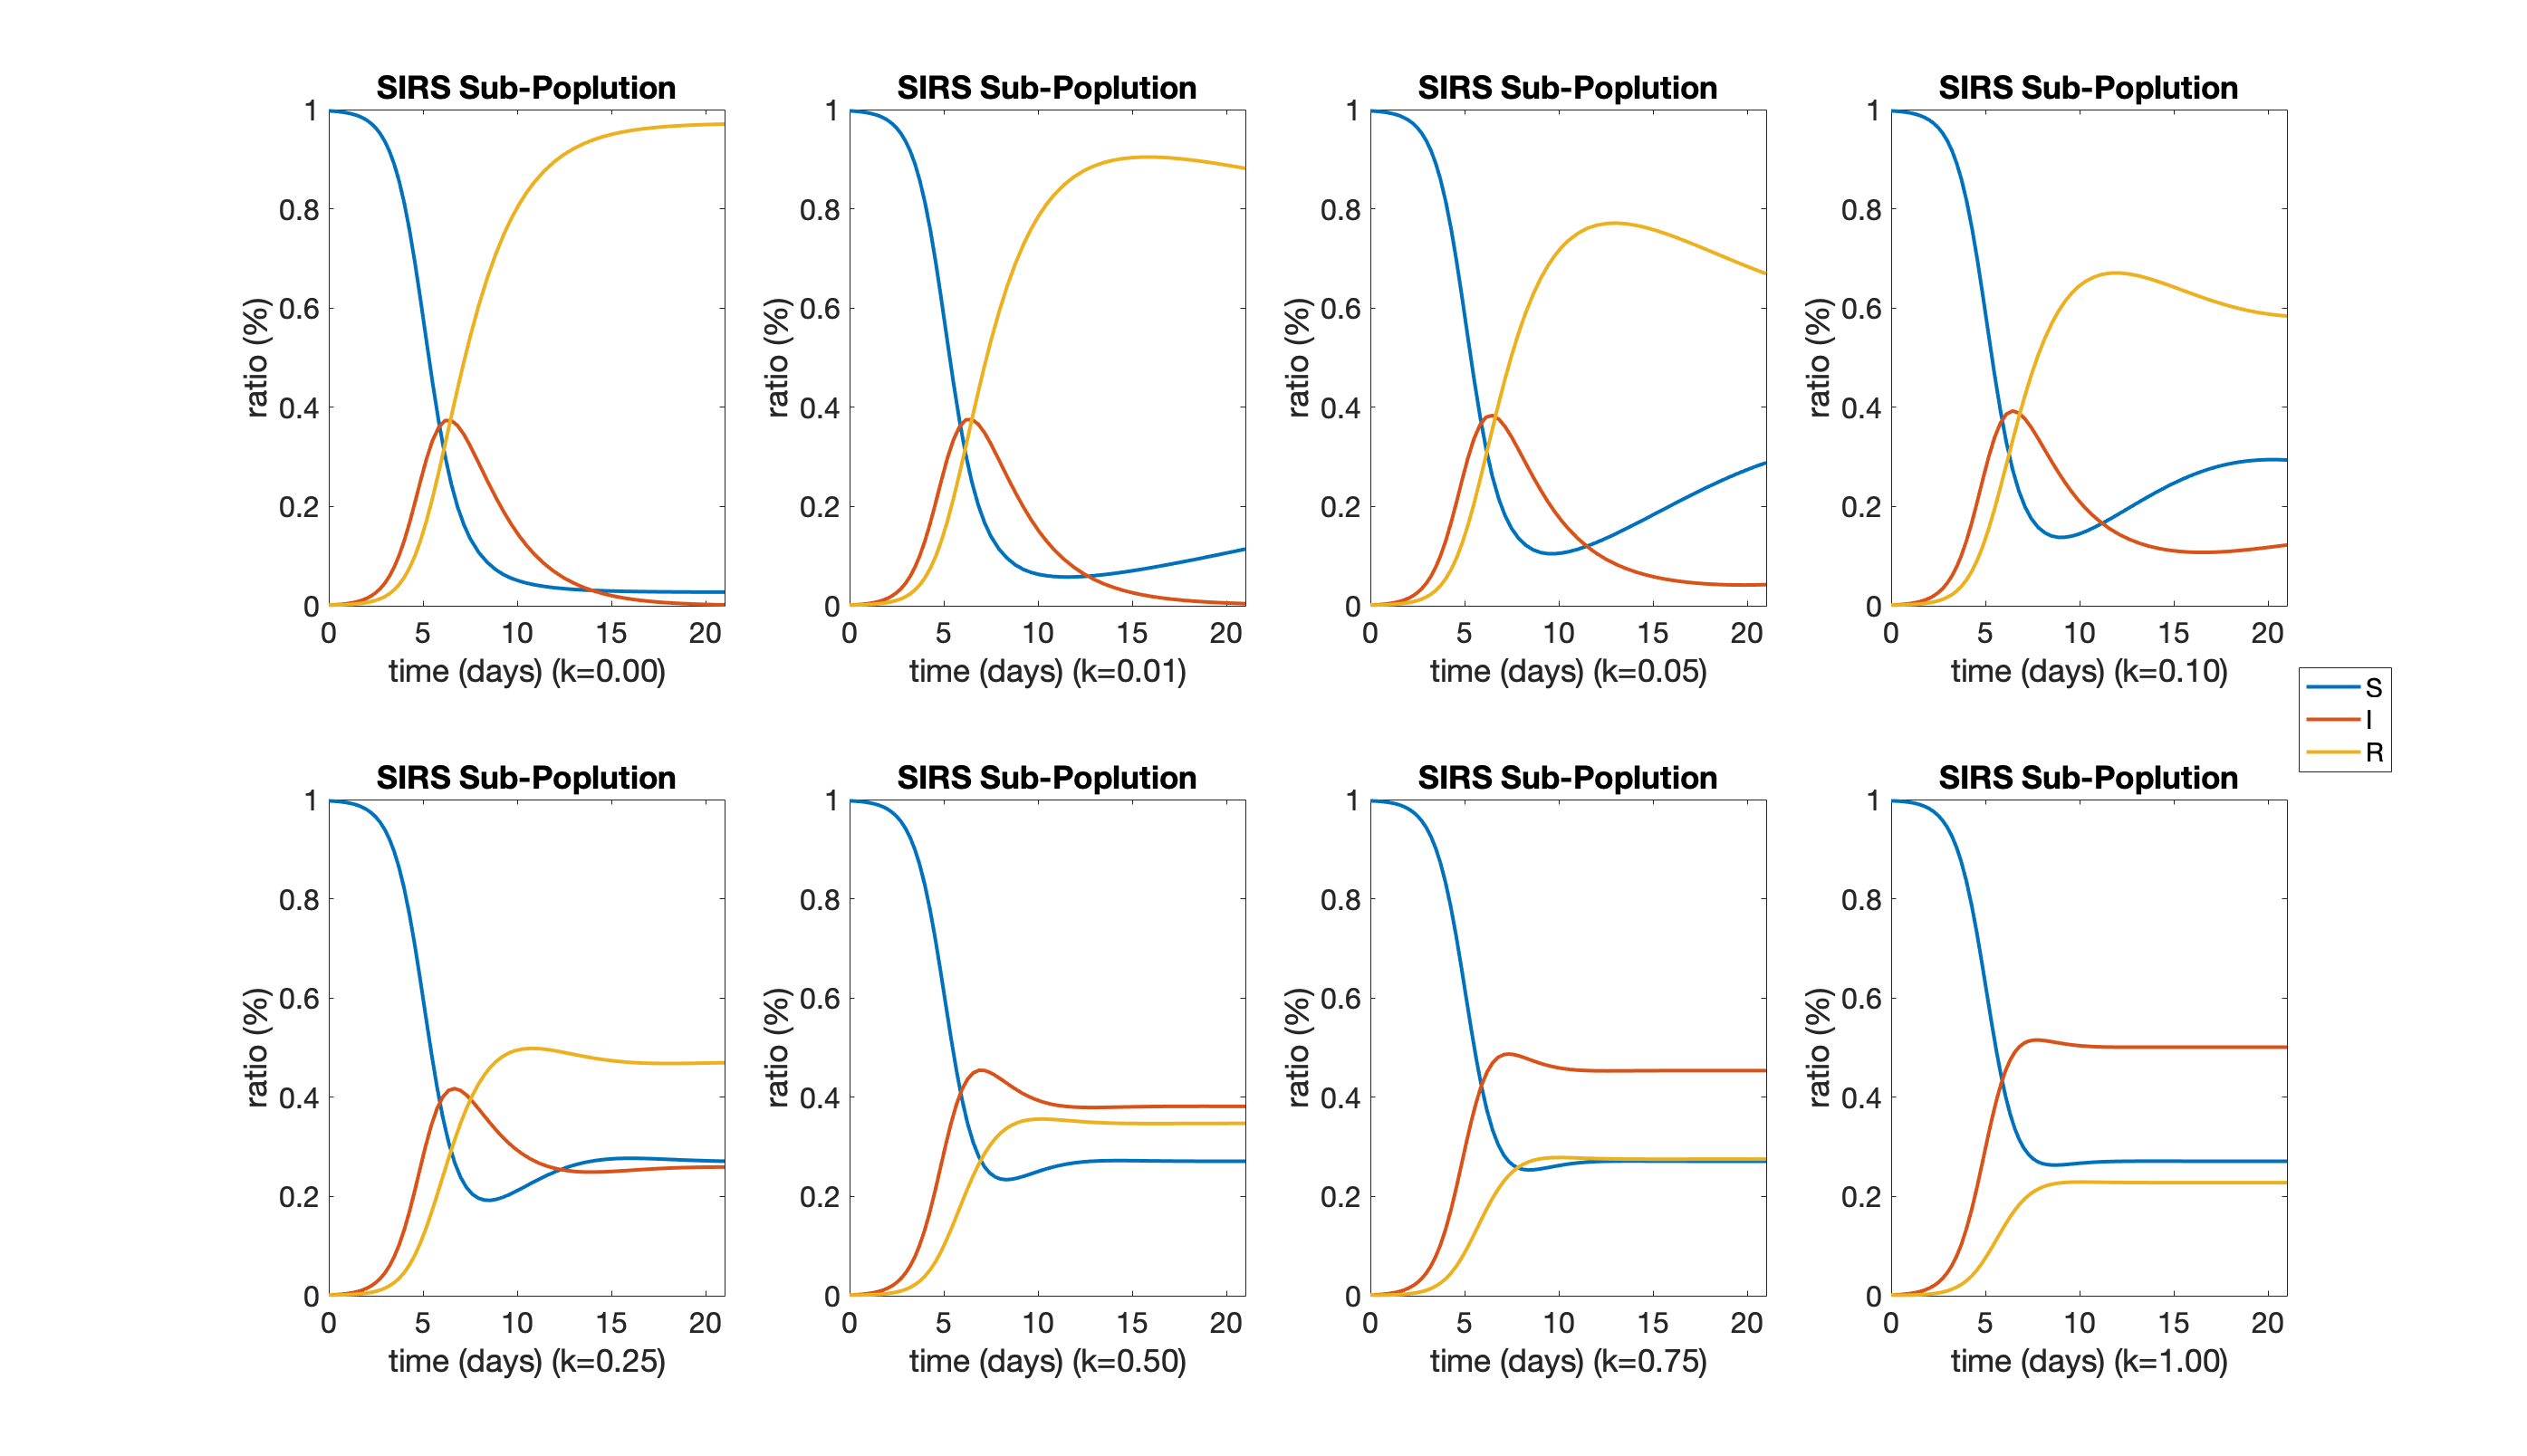
\includegraphics[width=\textwidth]{hw10_8_b1.png}
    \caption{S, I, R population of SIRS model with different k}
\end{figure}

When $k>0.1$, SIRS system would reach equilibrium status after 10 days. As shown in the figure, if $k<0.5$, the number of recovery population is larger than the susceptible when converging; in contrast to the situation when $k>0.5$.We found that the population of $S$ and $R$ don't converge to equilibrium status after 30 days when recovery rate $k$ is small, such as $0<k<0.1$. Extend the time to \textbf{200} days. We find the curves would oscillate with period with decreasing magnitudes. The infection breaks out with round 70 days after the susceptible population peaks. According to the (d), the eigenvalues of Jacobian matrix has imaginary part when $a^2-4b<0; (let\ a=k+\alpha I_s;b=\alpha I_s(k+r))$. In this example, we always have the imaginary part in the eigenvalues, which means all the curves would have oscillations. When $k$ is larger, its frequency should be larger. But the magnitude of each peak attenuates quickly, resulting in the quck convergence for large $k$ (such as $k>0.5$). 

\begin{figure}[!ht]
    \centering
    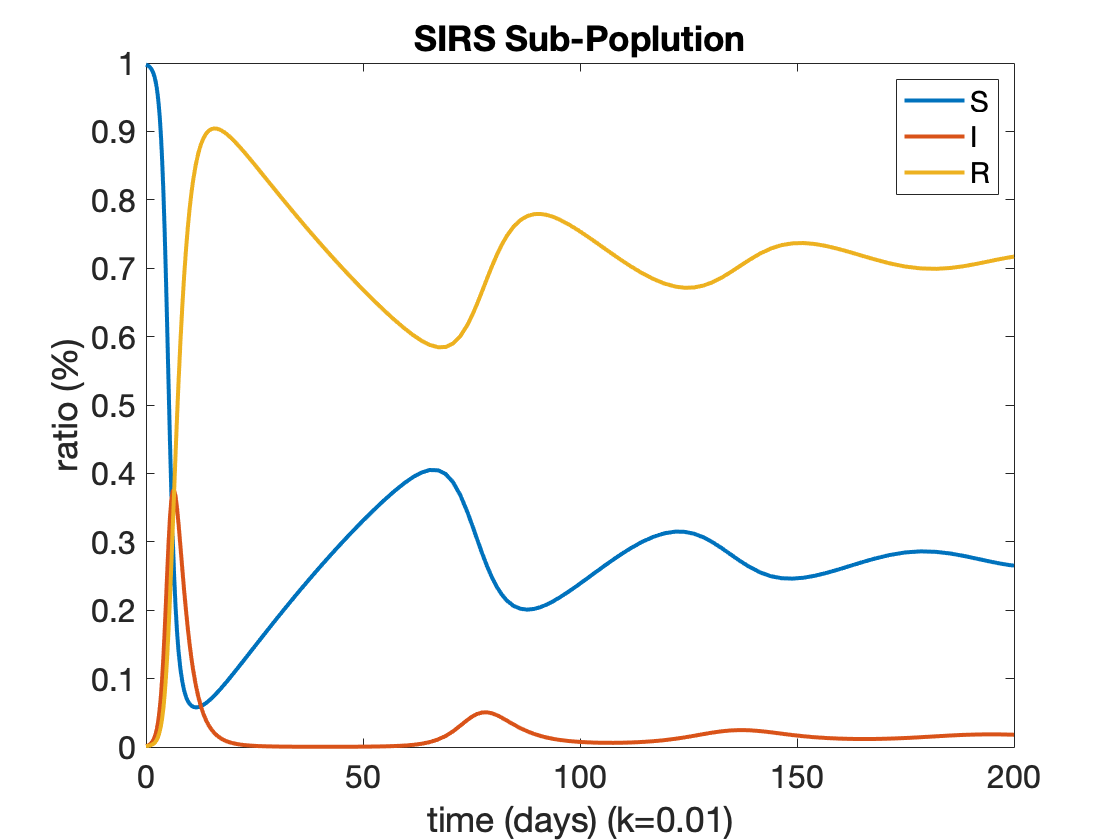
\includegraphics[width=0.8\textwidth]{hw10_8_b2.png}
\end{figure}

\textbf{(c)}
When reaching equilibrium point, \\
$\dot{S} =0= -\alpha SI+kR\\
\dot{I} =0= \alpha SI - \gamma I\\
\dot{R} =0= \gamma I - kR$

So one equilibrium point could be: \\
$I=0,R=0,S=N-I-R=N\rightarrow N_{s1}=\newvec{N\\0\\0}$

When $I\neq 0;R\neq 0$, $I/R=k/\gamma;S=\gamma/\alpha\rightarrow R=(N-\gamma/\alpha)/(1+k/\gamma);I=k/\gamma R=k(N-\gamma/\alpha)/(\gamma+k)$. So the other equilibrium point is:\\
$N_{s2}=\newvec{\gamma/\alpha\\k(N-\gamma/\alpha)/(\gamma+k)\\(N-\gamma/\alpha)/(1+k/\gamma)}$

\textbf{(d)}
As equation 10.46, For SIRS system, $\dot{I}=0=\alpha SI-\gamma I$ sets the lower bound. So the $R_0=\cfrac{N\alpha}{\gamma}$. 

The Jacobian matrix  of SIRS system is: \\
$\mathbf{A}=\newvec{-\alpha I_s&-\alpha S_s&k\\\alpha I_s&\alpha S_s-\gamma&0\\0&\gamma&-k}$\\
For $\det(\mathbf{A}-\lambda I)=0$, \\
$\mathbf{N}_{s1}: \lambda(k+\lambda)(\alpha N-\gamma-\lambda)=0\rightarrow \lambda_1=0;\lambda_2=-k;\lambda_3=\alpha N-\gamma$ \\
$\mathbf{N}_{s2}: \lambda(\lambda^2+(k+\alpha I_s)\lambda+\alpha I_s (k+\gamma))=0\rightarrow$ let $a=k+\alpha I_s;b=\alpha I_s(k+r)$, we have $\lambda_1=0;\lambda_2=\cfrac{-a+\sqrt{a^2-4b}}{2};\lambda_3=\cfrac{-a-\sqrt{a^2-4b}}{2}$. 

\textbf{(1)} For the first equilibrium point $N_{s1}$, it has 2 real eigenvalues that $-k<0;\alpha N-\gamma<0\rightarrow R_0=\alpha N/\gamma<1$. 

\textbf{(2)} For the second equilibrium point $N_{s2}$, which is after the epidemic, the system has 2 imaginary values with its real part as $-a=-(k+\alpha I_s)=-(k\cfrac{R_0-k/\gamma}{1+k/\gamma}) < 0$, indicating the stability when the system is at the second equilibrium point. The system depends on engineering parameter $k/\gamma$, and $R_0$ and physical parameter $k$.

\textbf{I.} When $k=0.03$, $\lambda_{2,3}=-0.0528 \pm 0.1842i$. The small imaginary part means small oscillation frequency. So the time to go to the equilibrium point is quite long as shown in the following figure. \\
The maximum infection population rate is $I_{max}/N=0.3796\approx 38\%$ and the infection rate for equilibrium stautus is $I_{stable}/N=0.0447\approx 4.5\%$. The propotion of the infectious population is relatively low in the end. It's less likely to become an endemic. 

\textbf{II.} When $k=0.3$, $\lambda_{2,3}=-0.3931 \pm 0.4610i$. THe imaginary part increases compared with $k=0.03$. Its oscillation frequency increases and it reaches equilibrium point rapidly. But this time, $I_{max}/N=0.4252\approx 42.5\%$ and $I_{stable}=0.2896\approx 29\%$. The propotion is quite large, so it's likely to become an endemic. Note that the stable susceptible population rate has no relationship with $k$, and its value is $S_{stable}=0.271\approx 27\%$.

This finding meets the expection that an endimic would keep spreading within a relatively large population when the immunity effect is bad.

\begin{figure}[!ht]
    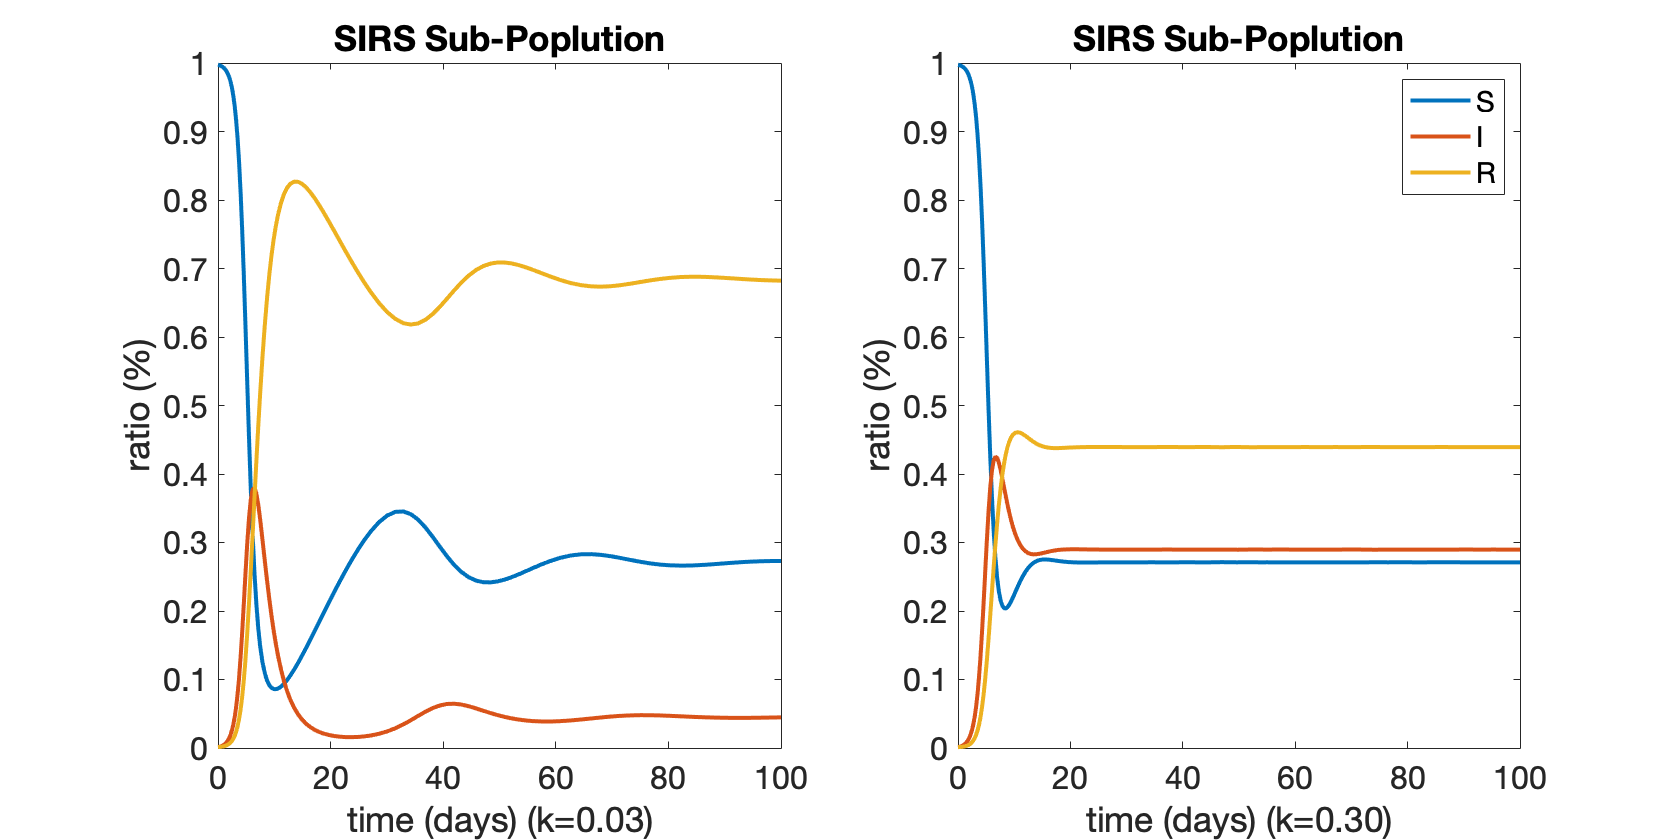
\includegraphics[width=\textwidth]{hw10_8_d.png}
    \caption{SIRS population in 100 days}
\end{figure}

\end{document}